\chapter{Processi primari}\label{Pp}
\section{Fornitura}			
Questo\glossario{processo}ha lo scopo di trattare le norme e i termini che i membri del gruppo\glossario{ZeroSeven}sono tenuti a rispettare per diventare fornitori della proponente Zero12 s.r.l e dei committenti Prof. Tullio Vardanega e Prof. Riccardo Cardin. \\
L'aspettativa del gruppo è instaurare e mantenere un rapporto di collaborazione costante con Zero12 s.r.l. per poter soddisfare al meglio i bisogni della Proponente e rispettare i vincoli richiesti.
\subsection{Studio di fattibilità} 
Dopo la presentazione dei \textit{capitolati$_{G}$}, è compito del \textit{Responsabile} convocare le riunioni necessarie per consentire al gruppo di esprimere idee e opinioni riguardo ai diversi capitolati. Le informazioni raccolte verranno utilizzate dagli \textit{Analisti} per redigere lo \textit{Studio di Fattibilità}. L'analisi si basa sui seguenti punti:
\begin{itemize}
	\item \textbf{Descrizione generale};
	\item \textbf{Finalità del progetto};
	\item \textbf{Tecnologie utilizzate};
	\item \textbf{Conclusione}.
\end{itemize}
\subsection{Rapporti di fornitura con la Proponente}
Durante l'intero progetto si intende instaurare un costante rapporto collaborativo con la Proponente, nella persona del Sig. Stefano Dindo, con il fine di:
\begin{itemize}
	\item determinare bisogni in modo più accurato possibile;
	\item scegliere in modo collaborativo i requisiti del prodotto;
	\item accordare insieme vincoli di qualità del prodotto;
	\item stimare tempi e costi.
\end{itemize}
A seguito della consegna del prodotto, salvo ulteriori accordi, non seguirà l'attività di manutenzione.
\subsection{Documentazione fornita}
\label{Documentazione fornita}
Di seguito viene indicata la documentazione che verrà fornita alla\glossario{Proponente}e al Committente con lo scopo di rendere trasparenti le scelte di:
\begin{itemize}
	\item \textbf{pianificazione}: \textit{Piano di Progetto};
	\item \textbf{processi}: \textit{Norme di Progetto};
	\item \textbf{verifica e validazione}: \textit{Piano di Qualifica};
	\item \textbf{obiettivi di qualità}: \textit{Piano di Qualifica};
	\item \textbf{requisiti}: \textit{Analisi dei Requisiti}.
\end{itemize}
%\paragraph{Piano di Progetto}
%Il \textit{Responsabile} si occupa della scrittura del \textit{Piano di Progetto} con l'obiettivo di organizzare le attività con efficienza e %misurare l'avanzamento del\glossario{progetto}, pertanto il documento in questione dovrà contenere:
%\begin{itemize}
%	\item \textbf{Analisi dei Rischi:} vengono analizzati sia i rischi, che potrebbero sorgere durante lo svolgersi del progetto, sia le %possibili soluzioni a questi rischi, tenendo conto dei relativi costi e delle scadenz
%	\item \textbf{Pianificazione:} si organizza nel dettaglio le attività da svolgere.
%	\item \textbf{Consuntivo di periodo e Preventivo a finire:} viene redatto il consultivo di periodo alla fine di ogni attività. In questo %modo si possono confrontare i risultati ottenuti con quelli attesi. Questi ultimi sono visibili nel preventivo, il quale contiene una stima %del lavoro necessario.
%\end{itemize}
%\paragraph{Piano di Qualifica}
%Gli \textit{Amministratori} documentano le norme per la\glossario{verifica}e la validazione dei prodotti e dei processi, la verifica avviene %con costanza affinché non vengano introdotti errori. Il documento contiene:
%\begin{itemize}
%	\item \textbf{Qualità di processo}: per garantire la qualità dei processi attraverso l'utilizzo di strumenti e metriche, inoltre è %necessario adottare come standard \textit{ISO/IEC 15504}.
%	\item \textbf{Qualità di prodotto}: per garantire e misurare la qualità dei prodotti sviluppati, è necessario adottare come standard %\textit{ISO/IEC 15010}.
%\end{itemize}

%\paragraph{Verbali Esterni}
%Vengono verbalizzati tutti gli incontri avvenuti con l'azienda Zero12 s.r.l., la redazione del verbale esterno è compito degli %\textit{Analisti}. I verbali esterni verranno inclusi nella documentazione fornita, inoltre si cercherà, ove possibile, di inviare una copia %del suddetto verbale all'azienda cliente.

\section{Sviluppo}
Il\glossario{processo}di sviluppo comprende tutte le attività e i compiti svolti dal gruppo per produrre il software richiesto dal \textit{proponente$_{G}$}.\\ Dallo sviluppo del\glossario{prodotto}ci si aspetta che questo soddisfi i test di verifica e di validazioni, gli obiettivi imposti e i bisogni della Proponente. Il processo di sviluppo si svolge secondo lo standard \textit{ISO/IEC 12207}.
\subsection{Analisi dei requisiti}
Gli \textit{Analisti} si occupano di analizzare nel dettaglio i\glossario{requisiti}che il prodotto finale dovrà soddisfare, il risultato viene poi documentato nell' \textit{Analisi dei Requisiti}. Vengono utilizzati i casi d'uso per l'analisi e la ricerca dei requisiti.
Il documento redatto dovrà rispettare le specifiche di seguito riportate.
\subsubsection{Fonti dei requisiti}
Compito di analisti è quello di redigere una lista di \textit{requisiti$_{G}$}. Tali requisiti possono essere ricavati da varie fonti, le quali sono:
\begin{itemize}
	\item \textbf{Capitolato}: i requisiti emersi dall'analisi del documento fornito dalla \textit{Proponente$_{G}$};
	\item \textbf{Verbali Esterni}: i requisiti emersi durante incontri con la Proponente;
	\item \textbf{Interni}: i requisiti emersi tramiti analisi e discussione interna del gruppo \textit{ZeroSeven$_{G}$};
	\item \textbf{Casi d'uso}: i requisiti emersi dall'analisi di uno o più casi d'uso.
\end{itemize}
\subsubsection{Classificazione dei requisiti}
Ogni\glossario{requisito}deve avere la seguente nomenclatura:
\begin{center}
	\textbf{R$\Bigl\{$A$\Bigr\}$$\Bigl\{$B$\Bigr\}$$\Bigl\{$XX$\Bigr\}$.$\Bigl\{$YY$\Bigr\}$}
\end{center}
dove:
\begin{itemize}
	\item \textbf{A:} corrisponde a uno dei seguenti requisiti:
	\begin{itemize}
		\item F: funzionale;
		\item Q: di qualità;
		\item P: di prestazione;
		\item V: di vincolo.
	\end{itemize}
	\item \textbf{B:} corrisponde a uno dei seguenti requisiti:
	\begin{itemize}
		\item O: obbligatorio;
		\item F: facoltativo;
		\item D: desiderabile.
	\end{itemize}
	\item \textbf{{XX}:} numero che identifica i \textit{requisiti$_{G}$};
	\item \textbf{{YY}:} numero progressivo che identifica i sottocasi, esso può, a sua volta, includere altri sottocasi.
\end{itemize}

\subsubsection{Casi d'uso}
Ogni caso d'uso deve presentare i seguenti campi:
\begin{itemize}
	\item Codice identificativo;
	\item Titolo
	\item Attori primari;
	\item Attori secondari (se presenti);
	\item Descrizione;
	\item Precondizione;
	\item Postcondizione;
	\item Flusso principale degli eventi.
\end{itemize}
Se un caso d'uso risulta essere particolarmente complesso allora viene corredato da un diagramma dei casi d'uso in linguaggio UML.
\subsubsection{Codice identificativo CU}
Ogni caso d'uso deve avere la seguente nomenclatura:
\begin{center}
	\textbf{UC$\Bigl\{$XX$\Bigr\}$.$\Bigl\{$YY$\Bigr\}$}
\end{center}
dove:
\begin{itemize}
	\item \textbf{UC:} Use Case;
	\item \textbf{{XX}:} numero che identifica i casi d'uso;
	\item \textbf{{YY}:} numero progressivo che identifica i sottocasi, esso può, a sua volta, includere altri sottocasi.
\end{itemize}


%\subparagraph{Diagrammi UML}
%Per la stesura dei diagrammi UML vengono adottate le seguenti convenzioni:
%\begin{itemize}
%	\item \textbf{Versione:} lo standard utilizzato per i grafici UML è la \textit{v2.0}.
%	\item \textbf{Lingua:} la lingua utilizzata è l'italiano.
%\end{itemize}


%\subparagraph{Requisiti}
%Ogni requisito deve presentare i seguenti campi:
%\begin{itemize}
%	\item Codice identificativo
%	\item Descrizione
%	\item Fonti
%\end{itemize}


\subsection{Progettazione} \label{progettazione}
%La progettazione deve poter dimostrare che tutti i\glossario{requisiti}specificati nell'\textit{Analisi dei Requisiti} siano rispettati. Per far %ciò, c'è bisogno della stesura dei seguenti documenti:
%\begin{itemize}
%	\item Specifica tecnica
%	\item Definizione di Prodotto
%\end{itemize}
\subsubsection{Scopo}
L'attività di Progettazione precede obbligatoriamente la produzione del software e consiste nel descrivere e fornire una soluzione al problema che sia soddisfacente per tutti gli \textit{stakeholders$_{G}$}. Essa serve a garantire che il prodotto sviluppato sia adeguato rispetto ai bisogni emersi nell'attività di Analisi. 
La progettazione permette di:
\begin{itemize}
	\item costruire l'architettura logica del prodotto;
	\item facilitare la codifica da parte dei \textit{Programmatori}, riducendo la complessità del problema originale, permettendo di organizzare i compiti e possibilmente facilitando la parallelizzazione;
	\item perseguire la correttezza per costruzione.
\end{itemize}
Come da \pianodiprogetto la Progettazione si svolgerà nell'arco di due periodi distinti. 
Nel primo di questi due periodi viene identificata una prima decomposizione logica dell'architettura, dopo aver opportunamente studiato i vari design patterns. Nel secondo la progettazione avviene in modo atomico e dettagliato, in modo che i \textit{Programmatori} possano implementare l'intero sistema nel modo più parallelo possibile. 
L'architettura dovrà soddisfare le seguenti qualità: 
\begin{itemize}
	\item \textbf{Sufficienza}: deve soddisfare i requisiti descritti nell'\textit{Analisi dei Requisiti v2.0.0};
	\item \textbf{Comprensibilità}: può essere compresa facilmente da tutti gli \textit{stakeholder$_{G}$};
	\item \textbf{Modularità}: deve essere suddivisa in parti chiare e ben distinte, ognuna con una singola responsabilità, perseguendo information hiding;
	\item \textbf{Robustezza}: è in grado di sopportare ingressi di tipi diversi, sia da parte dell'utente che dall'ambiente;
	\item \textbf{Flessibilità}: deve permettere modifiche a costi contenuti in caso di variazione dei requisiti;
	\item \textbf{Riusabilità}: deve permettere il riuso delle sue parti in altre applicazioni;
	\item \textbf{Efficienza}: deve utilizzare il minor numero di risorse possibili, in termini di tempo e spazio;
	\item \textbf{Affidabilità}: deve garantire di rispettare le sue specifiche di funzionamento nel tempo;
	\item \textbf{Disponibilità}: deve essere possibile effettuare manutenzione in tempi ridotti, possibilmente senza rendere indisponibile l'intero sistema;
	\item \textbf{Sicurezza}: deve essere esente da gravi malfunzionamenti e non deve essere vulnerabile a intrusioni;
	\item \textbf{Semplicità}: ogni parte contiene solo il necessario;
	\item \textbf{Incapsulazione}: le componente devono essere progettate in modo da nascondere dettagli implementativi;
	\item \textbf{Coesione}: le parti con un obiettivo comune devono stare insieme;
	\item \textbf{Basso accopiamento}: parti distinte devono dipendere poco o niente tra di loro.
\end{itemize}
\subsubsection{Diagrammi}
Al fine di rendere chiare e comprensibili le scelte progettuali effettuate e ridurre le possibili ambiguità, sarà necessario fare largo uso di vari tipi di diagrammi\glossario{UML}2.0, quali:
\begin{itemize}
	\item \textbf{Diagrammi delle classi}: descrivono i tipi di oggetti che fanno parte di un sistema mettendone in evidenza le relazioni statiche;
	\item \textbf{Diagrammi di sequenza}: descrivono la collaborazione di un gruppo di oggetti che devono implementare collettivamente un comportamento;
	\item \textbf{Diagrammi di attività}: descrivono il flusso di operazioni di un'attività attraverso la sua logica procedurale;
	\item \textbf{Diagrammi dei package}: descrivono un raggruppamento di un numero arbitrario di elementi (ad esempio classi) in un'unica unità ad alto livello.
	
\end{itemize}


\subsection{Diagrammi delle classi}
\label{DiagrammiDelleClassi}
Lo scopo del diagrammi delle classi può essere riassunto in:
\begin{itemize}
	\item Descrizione e definizione del tipo degli oggetti che fanno parte di un sistema;
	\item Descrizione e definizione delle relazioni statiche fra i tipi degli oggetti.
\end{itemize}
Le norme di seguito riportare valgono sia per \textit{Kotlin}, sia per \textit{NodeJS}.
\\
Ogni classe viene rappresentato come un rettangolo diviso in tre sezioni:
\begin{itemize}
	\item \textbf{Nome classe}: deve essere univoco, in notazione \glossario{CamelCase}, in inglese;
	\item \textbf{Attributi}: elenco campi dati della classe, secondo la notazione \texttt{visibility name : type}. Il modificatore di accesso deve essere inserito obbligatoriamente e deve essere uno dei seguenti:
	\begin{itemize}
		\item \textbf{+}: visibilità pubblica;
		\item \textbf{-}: visibilità privata;
		\item \textbf{\#}: visibilità protetta.
	\end{itemize}
	\item \textbf{Operazioni}: elenco dei costruttori, modificatori e metodi di quel tipo, utilizzando la sintassi \texttt{visibility operationName(value: type) : type }.
\end{itemize}
Nel caso in cui una classe non dovesse contenere campi dati e/o metodi, apparirà nel diagramma comunque, seppur vuota, la sezione ad essi dedicata. 
\begin{figure}[h]
	\centering
	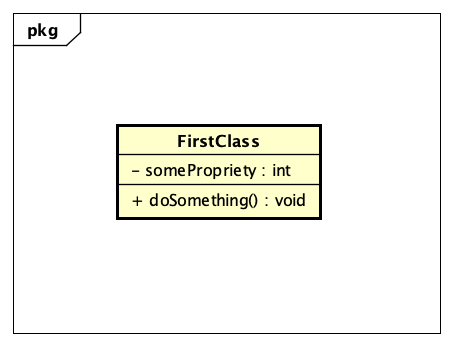
\includegraphics[scale=0.5]{images/SchemaClasse.png}
	\caption{Esempio diagramma di una classe}\label{}
\end{figure}
Nel caso di classi astratte il nome della stessa sarà scritto in corsivo.
\begin{figure}[h]
	\centering
	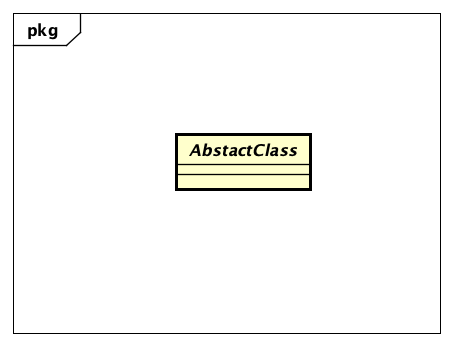
\includegraphics[scale=0.5]{images/ClasseAstratta.png}
	\caption{Esempio diagramma di una classe astratta}\label{}
\end{figure}
Aderendo alla sintassi UML2.x un'interfaccia viene rappresentata con cerchio vuoto con al di sotto il nome dell'interfaccia e l'elenco di operazioni.
\begin{figure}[h]
	\centering
	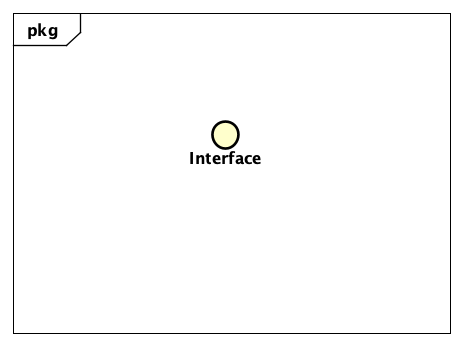
\includegraphics[scale=0.5]{images/Interfaccia.png}
	\caption{Esempio diagramma di un'interfaccia}\label{}
\end{figure}
I diagrammi delle classi sono collegati fra loro da frecce che esplicitano le dipendenze. In particolare, verranno considerati i seguenti tipi di freccia:
\begin{itemize}
	\item Freccia semplice: da classe A a classe B: indica che la classe A ha fra i propri campi dati una o più istanze della classe B;
	\begin{figure}[h]
		\centering
		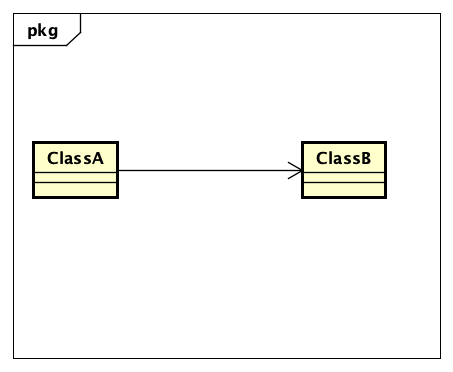
\includegraphics[scale=0.5]{images/Dipendenza.png}
		\caption{Relazione di dipendenza forte in un diagramma delle classi}\label{}
	\end{figure}
	\item Freccia tratteggiata, da classe A a classe B: indica una dipendenza, significa che A dipende da B secondo una primitiva che viene indicata al di sopra della freccia;
	\begin{figure}[h]
		\centering
		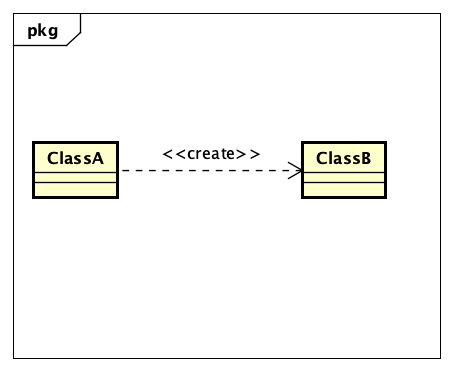
\includegraphics[scale=0.5]{images/Primitiva.png}
		\caption{Relazione di dipendenza debole in un diagramma delle classi}\label{}
	\end{figure}
	\item Freccia a diamante vuota, da classe A a classe B: indica un'aggregazione, una relazione non forte ovvero una relazione nella quale le classi che che ne prendono parte hanno entrambe significato anche prese in modo singolo;
	\begin{figure}[h]
		\centering
		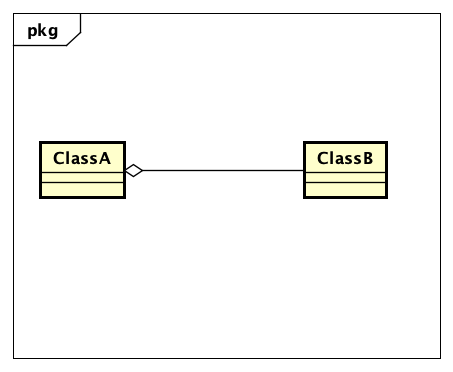
\includegraphics[scale=0.5]{images/Aggregazione.png}
		\caption{Relazione di aggregazione in un diagramma delle classi}\label{}
	\end{figure}
	\item Freccia a diamante piena, da classe A a classe B: indica la composizione, una relazione forte dove un'istanza della classe contenuta ha senso solo se esiste un'istanza della classe che contiene;
	\begin{figure}[h]
		\centering
		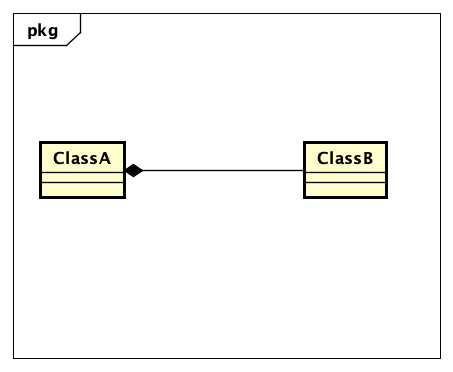
\includegraphics[scale=0.5]{images/Composizione.png}
		\caption{Relazione di composizione in un diagramma delle classi}\label{}
	\end{figure}
	\item Freccia vuota, da classe A a classe B: indica ereditarietà ed è il grado massimo di dipendenza fra classi. Indica che un oggetto A è anche un oggetto di tipo B.
	\begin{figure}[h]
		\centering
		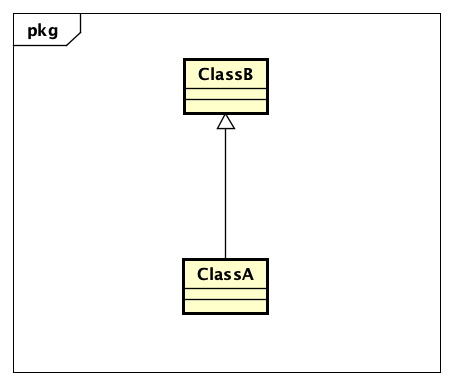
\includegraphics[scale=0.5]{images/Ereditarieta.png}
		\caption{Relazione di ereditarietà in un diagramma delle classi}\label{}
	\end{figure}
\end{itemize}



\subsection{Diagrammi di sequenza}
\label{DiagrammiSequenza}
I diagrammi di sequenza descrivono la collaborazione di un gruppo di oggetti che devono implementare collettivamente un comportamento. Ogni diagramma di sequenza avrà un senso di lettura verticale dall'alto al basso, verso che indica lo scorrere del tempo. I partecipanti vengono rappresentati tramite un rettangolo, al cui interno si trova un nome per identificarli rispettando la sintassi \texttt{name : Class}. Al di sotto di ogni istanza si trova la linea della vita. In ogni linea della vita ci sarò una barra di attivazione che indica in quale momento un partecipante è attivo. Da una barra di attivazione partono delle frecce, che rappresentano un messaggio, verso la linea della vita di oggetti già istanziati o, in alternativa, verso un nuovo partecipante per crearlo. 
In particolare , vengono utilizzati i seguenti tipi di frecce:
\begin{itemize}
	\item Freccia piena, per rappresentare un messaggio sincrono: corrisponde alla classica chiamata di un metodo, dove il chiamante rimane in attesa di una risposta. Sopra questa freccia si deve specificare il metodo chiamato rispettando la sintassi \texttt{method(param)};
	\item  Freccia, per indicare un messaggio asincrono: il chiamante non resta in attesa di risposta;
	\item Freccia tratteggiata, per indicare il messaggio di ritorno. Sopra questa freccia va indicato il tipo che viene ritornato;
	\item Freccia tratteggiata sormontata da << create >>: indica la creazione di un nuovo oggetto e termina sempre in un partecipante (rettangolo);
	\item Freccia piena sormontata da << destroy >>: indica la distruzione di un oggetto e termina sempre in una X, nella quale termina anche la linea della vita di un oggetto.
\end{itemize}

\subsection{Diagrammi di attività}
\label{DiagrammiAttivita}
I diagrammi di attività descrivono la logica procedurale decomponendo un'attività in un insieme di azioni. Essi contengono i seguenti elementi collegati sempre da frecce, che vengono indicati come mostrato di seguito:
\begin{itemize}
	\item \textbf{Nodo iniziale:} rappresentato da un pallino pieno. Indica il punto da cui inizia l'attività;
	\item \textbf{Activity:} raffigurata come un rettangolo che ne contiene una breve descrizione;
	\begin{figure}[h]
		\centering
		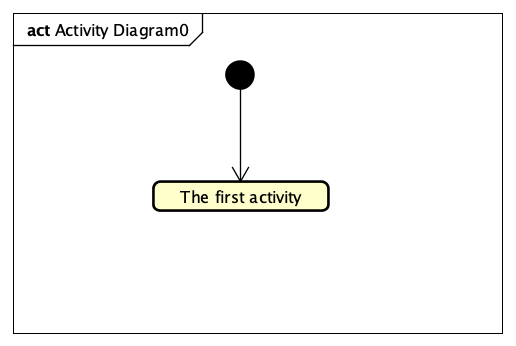
\includegraphics[scale=0.5]{images/PrimaActivity.png}
		\caption{Rappresentazione di un nodo iniziale e attività in un diagramma}\label{}
	\end{figure}
	\item \textbf{Fork:} rappresentato da una linea lunga verticale od orizzontale, indica un punto in cui l'esecuzione si parallelizza senza alcun vincolo temporale fra attività di processi differenti;
	\item \textbf{Join:} rappresentato da una linea lunga verticale od orizzontale, indica un punto in cui avviene la sincronizzazione fra processi paralleli;
		\begin{figure}[h]
		\centering
		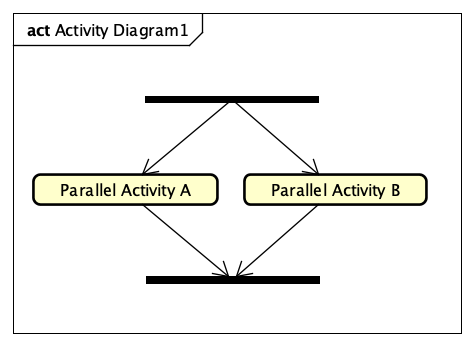
\includegraphics[scale=0.5]{images/ForkJoin.png}
		\caption{Esempio di Fork e Join in un diagramma di attività}\label{}
	\end{figure}
	\item \textbf{Branch:} rappresentato da un rombo con una freccia in ingresso. Indica un punto in cui si può prendere una decisione e seguire solo uno dei rami, ognuno dei quali deve avere la guardia nel formato \texttt{[guardia]};
	\item \textbf{Merge:} rappresentato da un rombo con una freccia in uscita. Indica il punto in cui i rami generati da un Branch si uniscono;
	\begin{figure}[h]
		\centering
		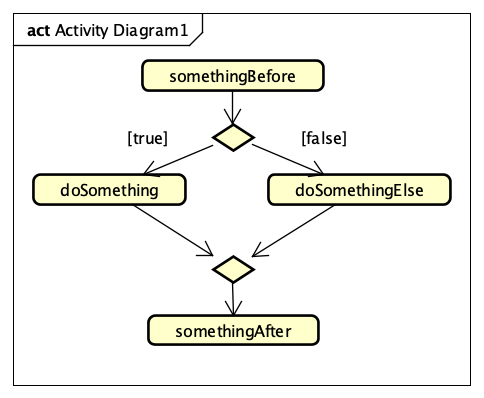
\includegraphics[scale=0.5]{images/BranchMerge.png}
		\caption{Esempio di Branch e Merge in un diagramma di attività}\label{}
	\end{figure}
	\item \textbf{Pin:} rappresentato da un quadrato piccolo dove entrano o escono frecce dalle Activity. Indica il passaggio di un parametro, il cui tipo va indicato a fianco con la sintassi \texttt{type};
	\item \textbf{Segnali:} rappresentati da due figure ad incastro, la prima per l'emissione del segnale, la seconda per la ricezione dello stesso e bloccante;
	\item  \textbf{Timeout:} rappresentato da una clessidra, serve per indicare timeout o eventi ripetuti. I timeout hanno frecce entranti e frecce uscenti, mentre gli eventi ripetuti hanno solo frecce uscenti;
	\item \textbf{Partizioni:} rappresentate da dei grandi rettangolo che dividono il diagramma, forniscono una responsabilità all'esecuzione delle azioni;
	\item \textbf{Regioni di espansione:} rappresentate da un rettangolo con i bordi tratteggiati, con degli argomenti in entrata e in uscita,  indica la ripetizione delle attività su una collezione di elementi;
	\item \textbf{Nodo di fine flusso:} rappresentato da un cerchio vuoto con una X al centro, indica un punto in cui uno dei rami di esecuzione muore, ma l'esecuzione prosegue negli altri rami;
	\item \textbf{Nodo finale:} rappresentato da due cerchi concentrici di cui il più esterno vuoto, indica il punto in cui l'esecuzione termina.
	
	\subsection{Diagrammi dei package}
	\label{DiagrammiPackage}
	Ogni package viene rappresentato attraverso un rettangolo con un'etichetta per il nome, che può contenere eventuali sotto-package. Le dipendenze tra i vari package vengono segnalate attraverso una freccia tratteggiata. Tale freccia, disegnata dal package A al package B, indica una dipendenza di A nei confronti di B.
	\begin{figure}[h]
		\centering
		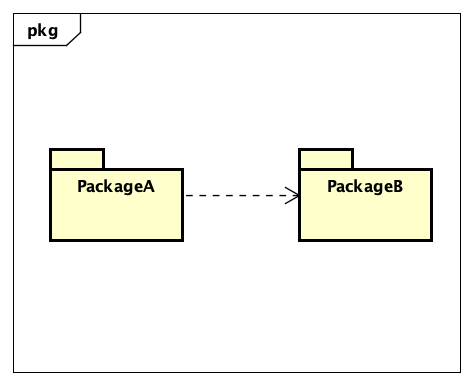
\includegraphics[scale=0.5]{images/DiagrammaPackage.png}
		\caption{Esempio di diagramma di package con dipendenza}\label{}
	\end{figure}
	
	
\end{itemize}
%\subsection{Integrazione}
%L'integrazione continua avviene mediante l'azione congiunta di\glossario{Travis-CI}e \textit{SonarQube$_{G}$}:ad ogni modifica %vengono eseguiti script automatici per il controllo della qualità del codice, il risultato di ogni build viene notificata ai membri del %gruppo tramite il canale\glossario{Slack}dedicato.

\subsection{Codifica}
Questa attività segue la Progettazione e consiste nell'implementazione effettiva di quanto precedentemente progettato. Per lo sviluppo dell'applicazione Android è stato deciso di utilizzare il software \textit{Android Studio$_{G}$}.
\subsubsection{Suddivisione dei package dell'applicazione}
Con riferimento al sito elencato nella sezione \ref{package}, la suddivisione dei file sorgente per package avverrà nel modo seguente:

\begin{itemize}
	\item	\textbf{com.megalexa:} rappresenta il package contenente tutti i file relativi all'applicazione;
	\item	\textbf{ui:} contiene tutti i package relativi all'interfaccia grafica;
		\subitem  \textbf{activities:} contiene tutti file contenenti le\glossario{activities}dell'applicazione.
		\subitem  \textbf{adapters:} conterrà tutti gli\glossario{adapters}che alcuni widget particolari di android richiedono (come le RecyclerView e le ListView);
		\subitem  \textbf{fragments:} contiene i file riguardanti i\glossario{fragments}prodotti dalle activities;
		\subitem	\textbf{util:} contiene interfacce utili per la realizzazione di interazioni particolari tra l'utente e l'interfaccia grafica;
	\item  \textbf{viewModel:}	contiene tutti i file che compongono il \textit{ViewModel$_{G}$}, che mette in comunicazione la parte grafica con quella logica;	
	\item  \textbf{models:} contiene tutti i file riguardanti la logica dell'applicazione;
		\subitem \textbf{connectors:} contiene tutti i file a supporto dei blocchi contenuti nel model: nello specifico, un connettore si rende necessario se il blocco a cui fa riferimento necessita di controlli aggiuntivi in rete per risultare corretto;
		\subitem \textbf{blocks:} contiene tutti i file riguardanti la logica dei blocchi che vanno a formare i workflow;
		\subitem \textbf{workflow:} contiene tutti i file riguardanti i workflow scelti dall'utente.
	
	\item  \textbf{util:} contiene tutte la classi di utilità definite nel corso dello sviluppo.
		\subitem\textbf{network:} contiene file che effettuano chiamate ad API esterne.
		\subsubitem\textbf{service:} contiene i file che realizzano l'integrazione ad \textit{API Gateway$_{G}$} effetuando le chiamate necessarie.
	

\end{itemize}
Sarà permesso definire ulteriori package all'interno di quelli sopra elencati, nel caso in cui ci sia bisogno di un maggiore dettaglio.
\subsubsection{Suddivisione dei package della skill}
	\begin{itemize}
		\item \textbf{MegAlexaSkill::lambda}: contiene il codice della skill MegAlexa che viene eseguito da AWS Lambda;
		\item \textbf{MegAlexaSkill::lambda::blocks}: contiene la parte di business della skill;
		\item \textbf{MegAlexaSkill::lambda::connection}: contiene le classi utili alla connessione e interfacciamento con il database;
		\item \textbf{MegAlexaSkill::node\_modules}: contiene tutte le dipendenze utili alla skill.
	\end{itemize}

\subsubsection{Stile di codifica: regole generali} 
Vengono elencate le norme alle quali i \textit{Programmatori} devono attenersi durante l'attività di programmazione e implementazione.
\begin{itemize}
	\item \textbf{Parentesi:} devono essere aperte utilizzando il metodo \textit{inline}, ovvero iniziano nella stessa riga del costrutto saltando uno spazio, inoltre blocchi di codice vanno racchiusi tra parentesi graffe;
	\item \textbf{Univocità dei nomi:} il nome delle classi, dei metodi e delle variabili deve essere il più esplicativo possibile al fine di garantire una maggior comprensione;
	\item \textbf{Nomi delle costanti:} la definizione delle costanti deve essere fatta utilizzando solo lettere maiuscole.
	\item \textbf{Nomi delle classi:} il nome delle classi deve iniziare con la lettera maiuscola;
	\item \textbf{Nomi dei metodi:} il nome dei metodi deve iniziare con la lettera minuscola, se sono composti da più parole allora le parole successive iniziano con la lettera maiuscola;
	\item \textbf{Lingua:} la lingua utilizzata è l'inglese, sia per i nomi delle classi, dei metodi e delle variabili, sia per i commenti del codice scritto.
\end{itemize}

\subsubsection{Utilizzo delle librerie}
\begin{itemize}
	\item Assicurarsi che le librerie utilizzate non presentino funzioni deprecate;
	\item assicurarsi che le versioni delle librerie utilizzate siano stabili (versioni 1.0.0 e successive);
	\item minimizzare il più possibile l'inclusione di librerie aggiuntive.
\end{itemize}

\subsubsection{Indentazione}
Viene definito il modo corretto di indentare il codice: l'apertura delle parentesi deve essere posta sulla stessa linea della dichiarazione a cui fa riferimento e separata da uno spazio.\\\\
\begin{minipage}{0.45\textwidth}
\begin{tabular}{p{\textwidth}}	
	\textbf{Corretto}
	\begin{lstlisting}
	
	private fun Foo() {
	\\contenuto
	}
	
	\end{lstlisting}
\end{tabular}
\end{minipage}
\hfill
\begin{minipage}{0.45\textwidth}
\begin{tabular}{|p{\textwidth}}

\textbf{Errato}
\begin{lstlisting}
	private fun Foo()
	{
	\\contenuto
	}

\end{lstlisting}
\end{tabular}

\end{minipage}


\subsubsection{Linee vuote} Lasciare righe vuote dopo i blocchi e prima di un nuovo statement. \\\\
\begin{minipage}{0.45\textwidth}
	\begin{tabular}{p{\textwidth}}	
		\textbf{Corretto}
		\begin{lstlisting}
	\\contenuto
		function a():Any {
		return bar
		}
		
		function b(): Any {
		return foo
		}
					
		\end{lstlisting}
	\end{tabular}
\end{minipage}
\hfill
\begin{minipage}{0.45\textwidth}
	\begin{tabular}{|p{\textwidth}}
		
		\textbf{Errato}
		\begin{lstlisting}
	\\contenuto
		function a():Any {
		return bar
		}	
		function b(): Any {
		return foo
		}
		\end{lstlisting}
	\end{tabular}
	
\end{minipage}
\subsubsection{Dichiarazione di variabili}

\paragraph{Kotlin}
In Kotlin vi è una distinzione fra variabili in sola lettura (\texttt{val}) e in lettura e scrittura(\texttt{var}). \'E opportuno scegliere accuratamente il tipo di variabile da dichiarare, e tutte devono seguire la seguente sintassi.
\begin{lstlisting}
val foo = Foo() 						
\end{lstlisting}

Se risulta necessario dichiarare una variabile come \texttt{lateinit}, specificare il tipo come segue
\begin{lstlisting}
lateinit val foo: Type							
\end{lstlisting}

Per dichiarare i campi dati di una classe, Kotlin fornisce una sintassi compatta che è opportuno seguire, l'inizializzazione dei campi dati deve avvenire mediante il costrutto \texttt{init}:

\begin{lstlisting}
class myClass(private val param1: Type,private val param2: Type) {	
	init {
	this.param1= param1
	this.param2= param2	
	} 
}
\end{lstlisting}

Le dichiarazioni di import vanno poste obbligatoriamente all'inizio del file:\\\\
\begin{minipage}{0.45\textwidth}
	\begin{tabular}{p{\textwidth}}	
		\textbf{Corretto}
		\begin{lstlisting}
		import java.util.*
		
		class example() {
		\\contenuto
		}
		\end{lstlisting}
	\end{tabular}
\end{minipage}
\hfill
\begin{minipage}{0.45\textwidth}
	\begin{tabular}{|p{\textwidth}}		
		\textbf{Errato}
		\begin{lstlisting}
		class example {
		\\contenuto
		}
		
		import java.util.*
		\end{lstlisting}
	\end{tabular}
	
\end{minipage}

\paragraph{Node.JS}
Le variabili globali e le dichiarazioni di \texttt{require} devono essere poste all'inizio del file:\\

\begin{minipage}{0.45\textwidth}
	\begin{tabular}{p{\textwidth}}	
		\textbf{Corretto}
		\begin{lstlisting}
		var axios = require("axios")
		
		class Example {
		\\contenuto
		}
		
		class SecondExample {
		\\contenuto
		}
		\end{lstlisting}
	\end{tabular}
\end{minipage}
\hfill
\begin{minipage}{0.45\textwidth}
	\begin{tabular}{|p{\textwidth}}		
		\textbf{Errato}
		\begin{lstlisting}
		class Example{
		\\contenuto
		}
		
		var axios = require("axios")
		
		class SecondExample {
		\\contenuto
		}
		\end{lstlisting}
	\end{tabular}
	
\end{minipage}
\newpage
La dichiarazione di \texttt{export} viene posta obbligatoriamente alla fine del file:\\

\begin{minipage}{0.45\textwidth}
	\begin{tabular}{p{\textwidth}}	
		\textbf{Corretto}
		\begin{lstlisting}
		\\contenuto
		class Example {
		\\contenuto
		}

		modules.export = Example;
		\end{lstlisting}
	\end{tabular}
\end{minipage}
\hfill
\begin{minipage}{0.45\textwidth}
	\begin{tabular}{|p{\textwidth}}		
		\textbf{Errato}
		\begin{lstlisting}
		\\contenuto
		modules.export = Example;
		\\contenuto
		class Example {
		\\contenuto
		}
		\end{lstlisting}
	\end{tabular}
	
\end{minipage}

\subsubsection{Parentesizzazione}

I blocchi di codice aventi una sola riga devono omettere le parentesi graffe:\\\\
\begin{minipage}{0.45\textwidth}
	\begin{tabular}{p{\textwidth}}	
		\textbf{Corretto}
		\begin{lstlisting}
		if(foo.isValid())
			return true
		
		\end{lstlisting}
	\end{tabular}
\end{minipage}
\hfill
\begin{minipage}{0.45\textwidth}
	\begin{tabular}{|p{\textwidth}}		
		\textbf{Errato}
		\begin{lstlisting}
		if(foo.isValid()) {
			return true
		}
		\end{lstlisting}
	\end{tabular}
	
\end{minipage}
\\\\\\
In presenza di blocchi annidati l'indentazione deve essere la seguente:\\

\begin{minipage}{0.45\textwidth}
	\begin{tabular}{p{\textwidth}}	
		\textbf{Corretto}
		\begin{lstlisting}
		class a() {
			\\contenuto		
			function b() {			
			\\contenuto
			}
			
			function c() {
			\\contenuto
			}
		}
		\end{lstlisting}
	\end{tabular}
\end{minipage}
\hfill
\begin{minipage}{0.45\textwidth}
	\begin{tabular}{|p{\textwidth}}
		\textbf{Errato}
		\begin{lstlisting}			
		class a() {
		\\contenuto		
		function b() {
		\\contenuto
		}
		function c() {
		\\contenuto
		}
		}
		\end{lstlisting}
	\end{tabular}
	
\end{minipage}
\paragraph{NodeJS}
La parentesizzazione di blocchi annidati deve seguire il seguente schema:\\

\begin{minipage}{0.45\textwidth}
	\begin{tabular}{p{\textwidth}}	
		\textbf{Corretto}
		\begin{lstlisting}
		class Example {
			constructor {
			\\contenuto
			}
			
			data() {	
				fetchData() {
				\\contenuto
				}	
			}
		}
		\end{lstlisting}
	\end{tabular}
\end{minipage}
\hfill
\begin{minipage}{0.45\textwidth}
	\begin{tabular}{|p{\textwidth}}
		\textbf{Errato}
		\begin{lstlisting}	
		class Example {
		constructor {
		\\contenuto
		}
		
		data() {	
			fetchData() {
			\\contenuto
			}	
		}
		}		
	
		\end{lstlisting}
	\end{tabular}
	
\end{minipage}
\subsubsection{Commenti}
Sfruttare il comando fornito da\glossario{JavaDoc}per fornire una descrzione accurata delle funzioni che vengono implementate.\\

\begin{minipage}{0.45\textwidth}
	\begin{tabular}{p{\textwidth}}		
		\textbf{Corretto}
		\begin{lstlisting}	
		/** fun()
		* description
		* description
		*/
		fun a():Unit {
		\\contenuto
		}	
		\end{lstlisting}
	\end{tabular}
\end{minipage}
\hfill
\begin{minipage}{0.45\textwidth}
	\begin{tabular}{|p{\textwidth}}		
		\textbf{Errato}
		\begin{lstlisting}
		\\description
		\\description
		\\description
		\\description
		fun a(): Unit {
		\\contenuto
		}
		\end{lstlisting}
	\end{tabular}
	
\end{minipage}
\\\\\\
JavaDoc inoltre mette a disposizione dei comandi aggiuntivi che permettono di identificare automaticamente i parametri e il tipo di ritorno delle funzioni:
\begin{itemize}
	\item \textbf{@param:} per fornire la descrizione di un parametro;
	\item \textbf{@return:} per fornire un dettaglio maggiore sul risultato della funzione;
	\item \textbf{@exception \textbackslash @throws:} descrive le eccezioni lanciate dai metodi;
	\item \textbf{@link:} per collegare un package o una classe a cui si fa riferimento.
\end{itemize}
\subsubsection{Codifica di XML}
\glossario{XML}viene utilizzato da kotlin per definire la disposizione degli oggetti grafici sullo schermo, vengono quindi definite le norme sull'indentazione del codice e l'annidamento dei tag.

\paragraph{Apertura e chiusura dei tag}
Nel caso in cui un tag non abbia figli, esso dovrà essere chiuso come segue:

\begin{lstlisting}
<exampletag />
\end{lstlisting}

In presenza di molteplici attributi lo stile di scrittura deve essere il seguente:

\begin{lstlisting}
<exampleTag 
		attribute1= "1"
		attribute2= "2"
		attribute3= "3"
		attribute4= "4"
		attribute5= "5"
/>
\end{lstlisting}

La presenza di tag annidati deve essere indentata nel seguente modo:
\begin{lstlisting}
<parentTag
		attribute1= "1"
		attribute2= "2"
		attribute3= "3"
		attribute4= "4"
		attribute5= "5"
> 
		<childTag1
				attribute1= "1"
				attribute2= "2"
		/>	
		<childTag2
				attribute3= "3"
				attribute4= "4"
				attribute5= "5"
		/>
</parentTag>
\end{lstlisting}

\paragraph{Dichiarazione di id e stringhe univoche} 
L'\textit{XML schema$_{G}$} adottato da Kotlin per definire i layout in XML permette di definire id univoci nel seguente modo: 

\begin{lstlisting}
<TextView
		android:id="@+id/idView"
/> s
\end{lstlisting}
e di definire le stringhe collegandole in un file separato chiamato \texttt{strings.xml}, in modo da permettere una facile conversione a una seconda lingua:
\begin{lstlisting}
<TextView
		android:text="@string/todo"
/> 
\end{lstlisting}
 è quindi obbligatorio definire id univoci e inserire componenti testuali come appena descritto.

\subsubsection{Intestazione}
L'intestazione di ogni file deve essere scritta nella seguente maniera: \\\\
/$^{*}$\\
$^{*}$ File: nome del file \\
$^{*}$ Version: versione del file \\
$^{*}$ Date: data di creazione del file \\
$^{*}$ Author: nome di crea e successivamente di chi modifica il file \\
$^{*}$ \\
$^{*}$ License: tipo di licenza \\
$^{*}$ \\
$^{*}$ History: registro delle modifiche \\
$^{*}$ Author $\vert$$\vert$ Date $\vert$$\vert$ Description \\
$^{*}$ \\
$^{*}$\textbackslash

\subsubsection{Versionamento}
Viene inserito all'interno dell'intestazione, descritta precedentemente, utilizzando la seguente nomenclatura:
\begin{center}
	\textbf{X.Y.Z}
\end{center}
dove:
\begin{itemize}
	\item \textbf{X:} rappresenta l'indice primario, l'avanzamento di questo corrisponde una maggior stabilità del file, inoltre comporta l'azzeramento dell'indice Y;
	\item \textbf{Y:} rappresenta l'indice di verifica, il suo incremento corrisponde a una verifica del file;
	\item \textbf{Z:}: rappresenta l'indice di modifica, il suo incremento corrisponde a una modifica del file.
\end{itemize}
La versione \textit{1.0.0} rappresenta un file completo e stabile in grado di essere testato, questo significa che le funzionalità obbligatorie sono state implementate e pertanto sono disponibili per essere testate.


